\documentclass{article}

\usepackage{url}
\usepackage{hyperref}
\usepackage{natbib}
\usepackage{changepage}
\usepackage{amsmath}
\usepackage[pdftex]{graphicx}
\def\mtt{\mathtt}
\def\mrm{\mathrm}
\usepackage[margin=1.4cm]{caption}
%\usepackage{aas_macros}
%\usepackage{multirow}

\def\mnras{MNRAS}

\begin{document}
\section{The MultiNest Algorithm}
The MultiNest algorithm is a Bayesian inference tool for parameter space exploration and model selection that has come to widespread use in Astrophysics and Cosmology over the past years. 

It builds upon the nested sampling technique producing the Bayesian evidence by integrating the likelihood associated with a given set of parameters over the multidimensional parameter space, and creates samples of the posterior distribution as a by-product.

The novel way in which MultiNest represents the sampled volume by an optimized set of ellipsoids makes it especially powerful for exploring multi-modal posteriors or posteriors with curving degeneracies in high dimensions.

Our implementation follows the full description of the algorithm in \cite{2009MNRAS.398.1601F}.
\section{Performance}
put comparison tables and colorful pictures here

\subsection{Test cases}

\subsubsection{The egg-box}

\subsubsection{Gaussian shells}

\subsubsection{Locate the lighthouse}

The following problem was taken from \cite{Siv2006}:

\vspace{0.2cm}

\begin{adjustwidth*}{1.2cm}{2.cm}
A lighthouse is somewhere off a piece of straight coastline at position $\alpha$ along the shore and a distance $\beta$ out to sea. It emits a series of highly collimated flashes at random intervals and hence random azimuths. These pulses are intercepted on the coast by photo-detectors that record only the fact that a flash has occurred, but not the angle from which it came. $N$ flashes have so far been recorded at positions \{$x_k$\}. Where is the lighthouses?
 \end{adjustwidth*}
 
 \vspace{0.2cm}
 
\noindent We are told $-2 < \alpha < 2$ and $0 < \beta < 2$, so we assume uniform priors for $\alpha$ and $\beta$ in these ranges. For a given flash measurement $x_k$, it can be shown that 

\begin{equation*}
\mrm{prob}(x_k | \alpha, \beta) = \frac{\beta}{\beta^2 + (x_k - \alpha)^2},
\end{equation*}

\noindent which says the probability that the $k^\mrm{th}$ flash will be measured at $x_k$, given the lighthouse is located at ($\alpha$, $\beta$), follows the Cauchy distribution. Thus, the likelihood function is given by

\begin{equation*}
\mathcal{L}(\alpha, \beta) = \prod_{k=1}^N \mrm{prob}(x_k | \alpha, \beta).
\end{equation*}

\noindent Simulated data of $N=64$ pulses are stored in {\tt lighthouse.dat} in the {\tt DataFiles} directory. With our program, we find $\alpha = 1.24 \pm 0.19$, $\beta = 0.97 \pm 0.16$, and $\log(\mathcal{Z}) =  -161.49 \pm 0.05$, which is consistent with \cite{Siv2006}. Figure \ref{fig:lighthouse} shows the joint posterior distribution for $\alpha$ and $\beta$. 

\begin{figure}[h]
\begin{center}
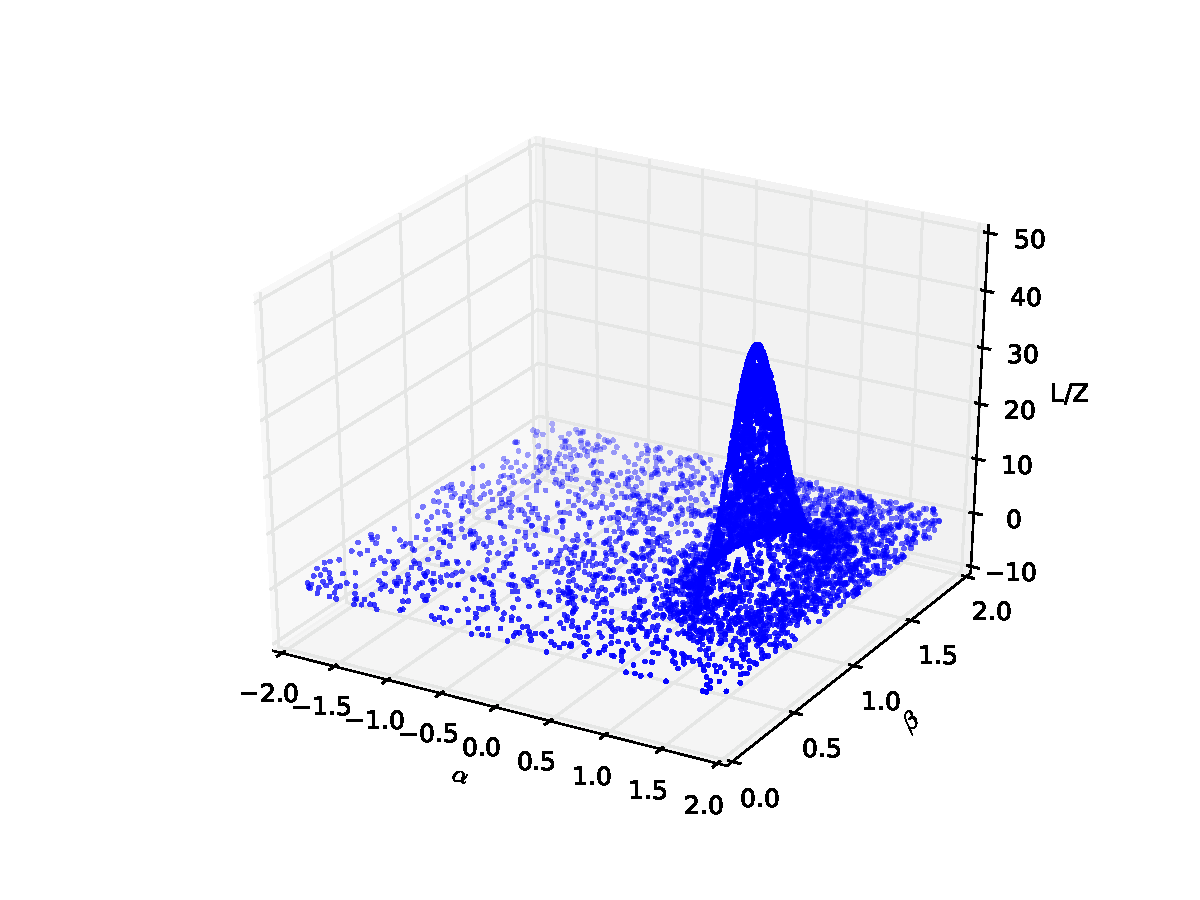
\includegraphics[width=12.0cm,trim=0cm 0cm 0cm 0cm,clip=true]{lighthouse.pdf}
\caption{Posterior probability distribution of the lighthouse location. We used 1000 active points.}
\label{fig:lighthouse}
\end{center}
\end{figure}

\section{User Instructions}
Compile the code using {\tt make}.  This program relies on the GNU Scientific Library (GSL) to do linear algebra, so be sure  you have GSL installed and that the compiler knows where to find its source files. Before running the program, run time parameters must be set in a file in the {\tt RunTimeFiles} directory. The format of run time files must be as follows. 

\begin{align*}
&\mtt{problem/data \ file}    &:& \ \ \mtt{problem \ or \ data \ file \ name}\\
&\mtt{N_{columns}}  	     &:& \ \ \mtt{\#}\\       
&\mtt{Dimension} 	            &:& \ \ \mtt{\# }\\
&\mtt{N_{points}}                &:& \ \ \mtt{\#}\\
&\mtt{efficiency \  \ factor}   &:& \ \ \mtt{1.0 \ (default \ vaule)}\\  
&\mtt{repartition \  \ factor}  &:& \ \ \mtt{1.2 \ (default \ value)}\\
&\mtt{\theta_1}                    &:& \ \ \mtt{prior \  \ \  \theta_{1,min}  \  \ \ \theta_{1,max}}\\     
&\mtt{\theta_2}                    &:& \ \ \mtt{prior \  \  \ \theta_{2,min}  \  \ \  \theta_{2,max}}\\     
\end{align*}

\noindent Here, $\theta_i$ is the $i^\mrm{th}$ parameter, {\tt prior} is the prior probability distribution for a given parameter, and the efficiency and repartition factors are optimization settings that are related to ellipsoidal partitioning and sampling. We have supplied three run time files for the test problems described above. The lighthouse problem is the only test case that requires data for likelihood evaluations, and its data file can be found in the {\tt DataFiles} directory. The current version of the code can only run these three problems, but we plan to adapt it for much more general use. 

The program takes the name of the run time file as a command-line argument. From the {\tt GrecoRothe\_MultiNest} directory, run the three test cases using the commands below.

\begin{adjustwidth*}{5cm}{3.5cm}
 {\tt 
 ./multinest eggbox.txt\\
./multinest gauss\_shells.txt\\
 ./multinest lighthouse.txt\\
 }
 \end{adjustwidth*}
 
\noindent If you would like to run make quick test runs with the code, lower the number of active points ({\tt Npoints}) in the run time files. Although our code can run the egg-box and Gaussian shells problems in an arbitrary number of dimensions, we have focused on 2 dimensions (2D), which allows for easy visualization and requires practical computation times. 

If the program runs successfully, it will output {\tt posterior\_pdfs.dat}, which has columns  $\theta_1$, $\theta_2$, log($\mathcal{L}$), and $\mathcal{L/Z}$. As the name implies, this file contains the necessary data to visualize the desired 2D posterior probability distributions. In addition, the program will output text similar to the following to the command-line. 

\begin{adjustwidth*}{1.2cm}{1.2cm}
{\tt
getting runtime parameters\\
creating 2000 active points in 2 dimensions\\
running MultiNest algorithm... this may take a few minutes\\
job complete!\\
**** results ****\\
number iterations = 34001\\
number reclusters = 2534\\
information: H =  8.9353 bits\\
global evidence: logZ = 235.683 +/- 0.0556484\\
****************}
\end{adjustwidth*}

As promised, the code tells us the evidence $\mathcal{Z}$, plus some additional information about how the algorithm is progressing. 

\bibliographystyle{plainnat}
\bibliography{writeup}

\end{document}
